
\documentclass[12pt, a4paper]{article}
\usepackage{fullpage}
\usepackage{graphicx}
\usepackage{wrapfig}
\usepackage{amsmath}
\usepackage{float}
\usepackage{listings}
\usepackage{lmodern}  % for bold teletype font
\usepackage{xcolor}   % for \textcolor

\definecolor{codegreen}{rgb}{0,0.6,0}
\definecolor{codegray}{rgb}{0.5,0.5,0.5}
\definecolor{codepurple}{rgb}{0.58,0,0.82}
\definecolor{backcolour}{rgb}{0.95,0.95,0.92}

\title{\textbf{EE2703 : Applied Programming Lab \\ Assignment 6}} % Title

\author{Potta Muni Asheesh \\ EE19B048} % Author name

\date{\today} % Date for the report

\begin{document}	
\lstset{
  language=Python,
  backgroundcolor=\color{backcolour},   
  commentstyle=\color{codegreen},
  keywordstyle=\color{magenta},
  numberstyle=\tiny\color{codegray},
  stringstyle=\color{codepurple},
  basicstyle=\ttfamily,
  breakatwhitespace=false,         
  breaklines=true,                 
  captionpos=b,                    
  keepspaces=true,                 
  %numbers=left,                    
  %numbersep=5pt,                  
  showspaces=false,                
  showstringspaces=false,
  showtabs=false,                  
  tabsize=2,
  columns=fullflexible,
  frame=single,
  postbreak=\mbox{\textcolor{red}{$\hookrightarrow$}\space},
}	
		
\maketitle % Insert the title, author and date

\section{Introduction}

1-dimensional model of tubelight is simulated using Python in this assignment. In a tubelight, electrons are emitted from the cathode and are accelerated in the tube. When they reach a certain velocity, they are capable of exciting electrons in other atoms to higher energy levels. When these excited atoms relax, they emit light. In this model, it is assumed that the atoms relax instantly. When the accelerated electrons excite other atoms, they lose their energy (i.e; velocity) and start accelerating again. Eventually, electrons reach the anode and are absorbed at the anode.

\section{Parameters involved in the simulation}

The tubelight is divided into \texttt{n} sections as finite memory is available in the computer. It is assumed that on an average \texttt{M} number of electrons enter the tubelight and the standard deviation of the same is \texttt{Msig}. \texttt{nk} is the number of turns the simulation is done. The threshold velocity to excite atoms is \texttt{u0} and the probability of an energised electron colliding with an atom is \texttt{p}. The user can provide these parameters through commandline arguments. The following are considered as the default parameters if none are given by the user.

\begin{lstlisting}
# Default values
n = 100  # number of sections the tubelight is divided into
M = 10   # mean of number of electrons injected per turn
Msig = 2 # std-dev of number of electrons injected per turn
nk = 500 # number of turns to simulate
u0 = 7   # threshold velocity
p = 0.5  # probability of ionization
\end{lstlisting}

\section{Simulation procedure}

\begin{itemize}
\item Electron information is stored in numpy arrays of dimension $nM$. For each electron, the information stored is, electron position (in \texttt{xx}), electron velocity (in \texttt{u}) and electron displacement in present turn (in \texttt{dx}). These arrays are updated in each turn.
\item After each turn, required information in accumulated in Python lists. The accumulated information is Intensity of emitted light (in \texttt{I}), electron position (in \texttt{X}) and electron velocity (in \texttt{V}).
\item Each space in the numpy arrays correspond to information regarding a particular electron. If it's position $x$ is greater than zero, then it means that the electron is present in the tubelight. \texttt{where} command is used to find these electrons' indices.
\begin{lstlisting}
existing = np.where(xx>0)[0]
\end{lstlisting}
\item It is assumed that the acceleration due to electric field is 1. So, the displacement of $i^{th}$ electron is given by
\begin{equation*}
dx_i = u_i \Delta t + \frac{1}{2} a (\Delta t)^2 = u_i + 0.5
\end{equation*}
Since the electric field acts only on electrons that are inside the tubelight, this operation is done only on the \texttt{existing} electrons. So, the position of these electrons change by the corresponding displacement. And, the electron's velocity increases by 1 unit.
\begin{lstlisting}
dx[existing] = u[existing] + 0.5
xx[existing] += dx[existing]
u[existing] += 1
\end{lstlisting}
\item Since, there are only $n$ sections of tubelight being simulated, if the position is greater than $n$, it means that the electron is absorbed by the anode. Again, \texttt{where} command is used to find these electrons and the positions, displacements and velocities of these electrons are set to 0.
\begin{lstlisting}
absorbed = np.where(xx > n)[0]
dx[absorbed] = 0
u[absorbed] = 0
xx[absorbed] = 0
\end{lstlisting}
\item The electrons which have velocity greater than the threshold velocity are found using \texttt{where} command and the probability of these electrons colliding with other atoms is given as $p$. So, the electrons which have collided with other atoms are found using \texttt{rand} command from module \texttt{np.random}. \texttt{rand} command creates an array of randon numbers between 0 and 1, this is used to find the electrons among the energetic which have collided and emitted light. The collided electrons come to rest after collision, so their velocity is set to 0.
\begin{lstlisting}
energetic = np.where(u >= u0)[0]
jj = np.where(np.random.rand(energetic.size) <= p)[0]
collided = energetic[jj]
u[collided] = 0
\end{lstlisting}
\item The collided electrons could have collided at any point between previous and present position. To find the actual point of collision, a random number  $\rho$,between 0 and 1, is generated and the actual position $x_i$ is found as given below.
\begin{equation*}
x_i \leftarrow x_i - dx_i \rho
\end{equation*}
\begin{lstlisting}
rho = np.random.rand(collided.size)
xx[collided] = xx[collided] - dx[collided]*rho
\end{lstlisting}
\item The positions where the electrons that have collided are stored in \texttt{I}.
\begin{lstlisting}
I.extend(xx[collided].tolist())
\end{lstlisting}
\item Now, the actual number of electrons that are newly injected is found as
\begin{lstlisting}
m = int(np.random.randn()*Msig + M)
\end{lstlisting}
These electrons are inserted in the empty spaces of array \texttt{xx}, where the position is 0. If there are not enough empty spaces, all the remaining empty spaces are filled. The electron position is set to 1.
\begin{lstlisting}
empty = np.where(xx == 0)[0]
m = int(min(m, empty.size))
xx[empty[:m]] = 1
\end{lstlisting}
\item In the beginning of the next iteration, the indices of all the existing electrons are found and their postions and velocities are stored in \texttt{X} and \texttt{V}.
\begin{lstlisting}
X.extend(xx[existing].tolist())
V.extend(u[existing].tolist())
\end{lstlisting}
\item The \textit{electron density, light emission intensity, electron phase space} plots are shown below.
\begin{figure}[H]
\centering
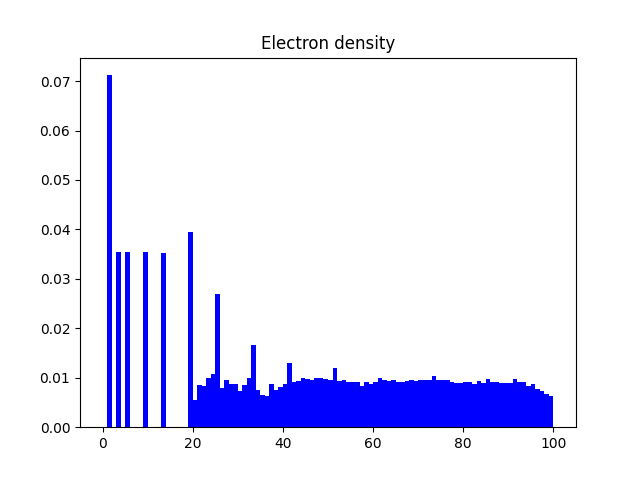
\includegraphics[width=0.8\textwidth]{Figure_1.png}
\caption{Electron density}
\end{figure}
\begin{figure}[H]
\centering
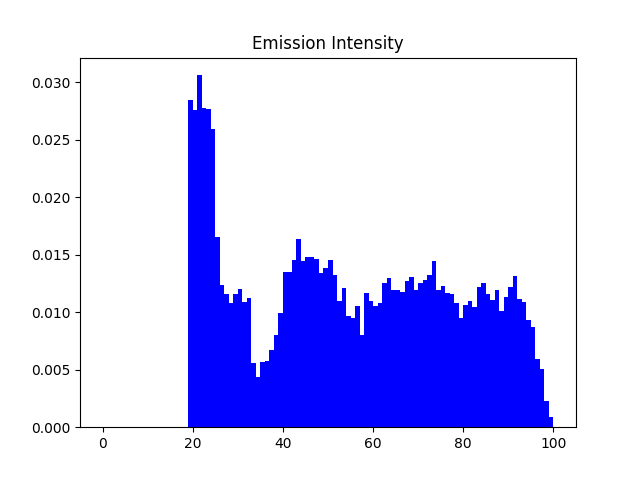
\includegraphics[width=0.8\textwidth]{Figure_2.png}
\caption{Emission intensity}
\end{figure}
\begin{figure}[H]
\centering
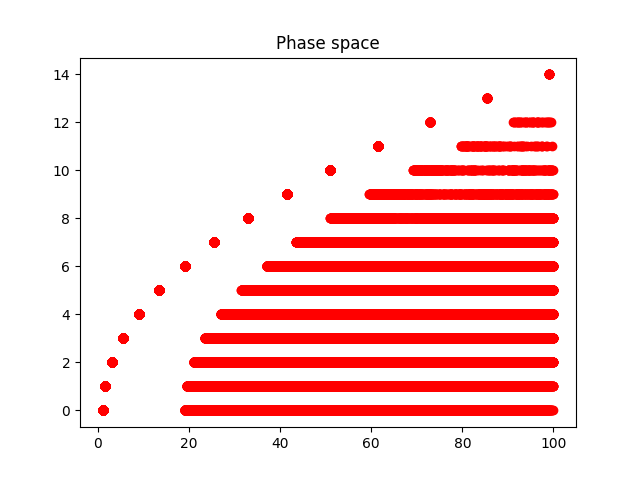
\includegraphics[width=0.8\textwidth]{Figure_3.png}
\caption{Electron phase space}
\end{figure}
\item The \texttt{hist} command not only plots the histogram, but will also return height level of each bar and also the x-axis values of bar edges. These can be used to find the x-positions of emissions and intensity at that position. The \textit{intensity data} can be printed in tabulted manner using \texttt{tabulate} module.
\begin{lstlisting}
count, bins = plt.hist(I, 100, color='blue', range=(0,100), density=True)[:2]

xpos = 0.5*(bins[:-1]+bins[1:])
print('Intensity data:')
print(tabulate(np.c_[xpos,count], headers=['xpos','count']))
\end{lstlisting}
The printed data is shown below.
\begin{verbatim}
Intensity data:
  xpos        count
------  -----------
   0.5  0
   1.5  0
   2.5  0
   3.5  0
   4.5  0
   5.5  0
   6.5  0
   7.5  0
   8.5  0
   9.5  0
  10.5  0
  11.5  0
  12.5  0
  13.5  0
  14.5  0
  15.5  0
  16.5  0
  17.5  0
  18.5  0
  19.5  0.0253764
  20.5  0.0277459
  21.5  0.028281
  22.5  0.0258351
  23.5  0.0262937
  24.5  0.0301154
  25.5  0.0178094
  26.5  0.0124589
  27.5  0.0138347
  28.5  0.0132233
  29.5  0.0114653
  30.5  0.0125354
  31.5  0.0115417
  32.5  0.00955438
  33.5  0.00573263
  34.5  0.00473897
  35.5  0.00611481
  36.5  0.0058855
  37.5  0.00657342
  38.5  0.00879003
  39.5  0.00886647
  40.5  0.0118474
  41.5  0.0132997
  42.5  0.0130704
  43.5  0.0150577
  44.5  0.0148284
  45.5  0.013529
  46.5  0.0153634
  47.5  0.0152106
  48.5  0.0143698
  49.5  0.0139112
  50.5  0.0146755
  51.5  0.0127647
  52.5  0.012994
  53.5  0.011771
  54.5  0.0113888
  55.5  0.00970725
  56.5  0.0110831
  57.5  0.0110066
  58.5  0.00955438
  59.5  0.0107009
  60.5  0.0107773
  61.5  0.0115417
  62.5  0.0113124
  63.5  0.011771
  64.5  0.00993656
  65.5  0.0132233
  66.5  0.0114653
  67.5  0.0136819
  68.5  0.0126118
  69.5  0.0133761
  70.5  0.0132997
  71.5  0.0132233
  72.5  0.0111595
  73.5  0.0108538
  74.5  0.0125354
  75.5  0.0116181
  76.5  0.0110066
  77.5  0.0136054
  78.5  0.012306
  79.5  0.00963082
  80.5  0.0104716
  81.5  0.0113124
  82.5  0.0107773
  83.5  0.0122296
  84.5  0.011771
  85.5  0.0132233
  86.5  0.0120767
  87.5  0.0106245
  88.5  0.0120003
  89.5  0.0113888
  90.5  0.011771
  91.5  0.0134526
  92.5  0.0123825
  93.5  0.00993656
  94.5  0.010013
  95.5  0.00703203
  96.5  0.00573263
  97.5  0.00366888
  98.5  0.00168157
  99.5  0.000611481
\end{verbatim}
\end{itemize}

\section{Conclusions}
\begin{itemize}
\item It is observed that, below position 20, the electron density peaks at discrete positions. This happens as discrete time steps are considered. But, after 20, there is continuous crowding of electrons, this is beacuse actual position of collision is found using random numbers. Also, after 20, the collision of electrons can happen at any position based on probability.
\item It is observed that there are no emissions before position 19-20. This is because, the electrons have to travel this distance to gain the threshold velocity required to excite the atoms.
\item A peak emission intensity is observed near positon 20, after that, the emissions decay. This is because the collided electrons need to travel some more distance to regain the threshold velocity.
\item In the electron phase space, discrete velocities are observed. Again, this is due to the discrete time consideration. The phase space is observed to be a family of parabolas. This can be explained as the acceleration is constant, the velocity-position relation is given by
\begin{equation*}
u^2 = 2a(x-x_0)
\end{equation*}
where $x_0$ is the position where the electron was at rest. $x_0$ is also the arbitrary constant in the family of parabolas. But $x_0$ is not quite arbitrary, since there can be any electrons at rest between positions 1 and 19-20. This explains the gap seen in the phase space plot.
\end{itemize}

\end{document} 
